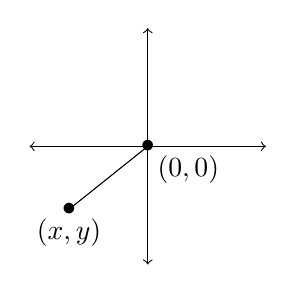
\begin{tikzpicture}
\draw[<->](-1.5,0)--(1.5,0);
\draw[<->](0,-1.5)--(0,1.5);
\draw(-1,-.8)node{$\bullet$}node[anchor=north]{$(x,y)$}--(0,0)node{$\bullet$}node[anchor=north west]{$(0,0)$};
\end{tikzpicture}
$(x,y)$ is a point such that $x<y<0$.  If a line is drawn
from $(x,y)$ to $(0,0)$, which of the following could be
the slope of the line?


\ifsat
	\begin{enumerate}[label=\Alph*)]
		\item $-3$
		\item $\frac{-4}{5}$
		\item $0$
		\item $\frac{1}{4}$%
	\end{enumerate}
\else
\fi

\ifacteven
	\begin{enumerate}[label=\textbf{\Alph*.},itemsep=\fill,align=left]
		\setcounter{enumii}{5}
		\item $-3$
		\item $\frac{-4}{5}$
		\item $0$
		\addtocounter{enumii}{1}
		\item $\frac{1}{4}$%
		\item $8$
	\end{enumerate}
\else
\fi

\ifactodd
	\begin{enumerate}[label=\textbf{\Alph*.},itemsep=\fill,align=left]
		\item $-3$
		\item $\frac{-4}{5}$
		\item $0$
		\item $\frac{1}{4}$%
		\item $8$
	\end{enumerate}
\else
\fi

\ifgridin
 $\frac{1}{4}$%

\else
\fi

